%%%%%%%%%%%%%%%%%%%%%%%%%%%%%%%%%%%%%%%%%%%%%%%%%%%%%%%%%%%%%%%%%%%%%%%%%%%%%%%%
%2345678901234567890123456789012345678901234567890123456789012345678901234567890
%        1         2         3         4         5         6         7         8

%\documentclass[journal,transmag]{IEEEtran}% Comment this line out if you need a4paper

\documentclass[10pt, conference]{ieeeconf}      % Use this line for a4 paper


\IEEEoverridecommandlockouts                              % This command is only needed if 
                                                          % you want to use the \thanks command

%\overrideIEEEmargins                                      % Needed to meet printer requirements.

% See the \addtolength command later in the file to balance the column lengths
% on the last page of the document

% The following packages can be found on http:\\www.ctan.org
%\usepackage{graphics} % for pdf, bitmapped graphics files
%\usepackage{epsfig} % for postscript graphics files
%\usepackage{mathptmx} % assumes new font selection scheme installed
%\usepackage{times} % assumes new font selection scheme installed
%\usepackage{amsmath} % assumes amsmath package installed
%\usepackage{amssymb}  % assumes amsmath package installed

\newtheorem{theorem}{Theorem}[section]
\newtheorem{lemma}[theorem]{Lemma}
\newtheorem{proposition}[theorem]{Proposition}
\newtheorem{corollary}[theorem]{Corollary}
\usepackage[ruled,vlined]{algorithm2e}
\usepackage{url}
\newenvironment{definition}[1][Definition]{\begin{trivlist}
\item[\hskip \labelsep {\bfseries #1}]}{\end{trivlist}}

\newcommand{\qed}{\nobreak \ifvmode \relax \else
      \ifdim\lastskip<1.5em \hskip-\lastskip
      \hskip1.5em plus0em minus0.5em \fi \nobreak
      \vrule height0.75em width0.5em depth0.25em\fi}

\def\lc{\left\lfloor}   
\def\rc{\right\rfloor}

\usepackage{amsmath,amssymb}

\usepackage{tabularx}
\usepackage{tikz,hyperref,graphicx,units}
\usepackage{subfigure}
\usepackage{benktools}
\usepackage{bbm}
\renewcommand{\baselinestretch}{.5}

\usepackage{caption}
\usepackage{epstopdf}
\renewcommand{\captionfont}{\footnotesize}
\usepackage{sidecap,wrapfig}
\usepackage[ruled,vlined]{algorithm2e}
\DeclareMathOperator*{\argmin}{arg\,min}
\DeclareMathOperator*{\argmax}{arg\,max}
\newcommand{\abs}[1]{\lvert#1\rvert} 
\newcommand{\norm}[1]{\lVert#1\rVert}
%\newcommand{\suchthat}{\mid}
\newcommand{\suchthat}{\ \big|\ }
\newcommand{\ba}{\mathbf{a}}
\newcommand{\bb}{\mathbf{b}}
\newcommand{\bc}{\mathbf{c}}
\newcommand{\bd}{\mathbf{d}}
\newcommand{\bg}{\mathbf{g}}
\newcommand{\bj}{\mathbf{j}}
\newcommand{\bn}{\mathbf{n}}
\newcommand{\bp}{\mathbf{p}}
\newcommand{\bw}{\mathbf{w}}
\newcommand{\bt}{\mathbf{t}}
\newcommand{\bu}{\mathbf{u}}
\newcommand{\by}{\mathbf{y}}
\newcommand{\bx}{\mathbf{x}}
\newcommand{\bz}{\mathbf{z}}
\newcommand{\bbf}{\mathbf{f}}
\newcommand{\bzero}{\mathbf{0}}
\newcommand{\bG}{\mathbf{G}}
\newcommand{\bA}{\mathbf{A}}
\newcommand{\bW}{\mathbf{W}}
\newcommand{\bX}{\mathbf{X}}
\newcommand{\mX}{\mathcal{X}}
\newcommand{\mD}{\mathcal{D}}
\newcommand{\mG}{\mathcal{G}}
\newcommand{\mN}{\mathcal{N}}
\newcommand{\mW}{\mathcal{W}}
\newcommand{\mF}{\mathcal{F}}
\newcommand{\bZ}{\mathbf{Z}}
\newcommand{\mR}{\mathcal{R}}

\newcommand{\bfc}{W}
\newcommand{\Qinf}{Q_{\infty}}
\newcommand{\st}[1]{_\text{#1}}
\newcommand{\rres}{r\st{res}}
\newcommand{\pos}[1]{(#1)^+}
\newcommand{\depth}{\operatorname{depth}}
\newcommand{\dist}{\operatorname{dist}}
\newcommand{\convhull}{\operatorname{ConvexHull}}
\newcommand{\minksum}{\operatorname{MinkowskiSum}}

\newcommand{\specialcell}[2][c]{ \begin{tabular}[#1]{@{}c@{}}#2\end{tabular}}
\newcommand{\acro}{SHIV}
\newcommand\independent{\protect\mathpalette{\protect\independenT}{\perp}}
\def\independenT#1#2{\mathrel{\rlap{$#1#2$}\mkern2mu{#1#2}}}

\newcolumntype{L}[1]{>{\RaggedRight\hspace{0pt}}p{#1}}
\newcolumntype{R}[1]{>{\RaggedLeft\hspace{0pt}}p{#1}}


\newboolean{include-notes}
\setboolean{include-notes}{true}
\newcommand{\adnote}[1]{\ifthenelse{ \boolean{include-notes}}%
 {\textcolor{blue}{\textbf{AD: #1}}}{}}
 
 \newcommand{\fpnote}[1]{\ifthenelse{ \boolean{include-notes}}%
 {\textcolor{blue}{\textbf{FP: #1}}}{}}
 
  \newcommand{\mlnote}[1]{\ifthenelse{ \boolean{include-notes}}%
 {\textcolor{purple}{\textbf{ML: #1}}}{}}

\renewcommand{\baselinestretch}{.95}
\usepackage{times}
\usepackage{microtype}
%\title{Iterative Imitation Learning with Reduced Human Supervision [v11]}
%\title{SHIV:  Reducing Human Supervision for Robot Active Learning [v11]}

\title{Robotic Grasping in Clutter}



\author{Wesley Hsieh, Dan Ricciardelli, Angela Hsueh}
\begin{document}


\maketitle
\thispagestyle{empty}
\pagestyle{empty}


\section{Introduction} 
Locating and grasping objects in a cluttered environment is an important problem that is relevant to many industrial applications such as shipment fulfillment in warehouses and manufacturing operations. Laskey et al explored learning policies for the grasping in clutter problem based on image data ~\cite{hierarchical_supervisors}. The paper used a hierarchy of supervisors to provide feedback to the robot, and demonstrated that a combination of supervisors of various performance and costs outperformed that of single supervisors. 

We explore changes in the properties of the experimental setup and their effects on the policy learned by the robot. In particular, we quantify the effect of different neural net architectures and image filters on the performance of the robot. We retrain the robot under the different configurations using DAgger ~\cite{ross2010reduction}, an imitation learning algorithm used in the original paper, and compare the performance of the resulting policies.

\section{Problem Statement}
We consider a robot grasping an object in a cluttered
environment. The robot's goal is to grasp a target, or goal,
object in the presence of extruded objects obstructing the
path towards the goal object. We do not assume knowledge of explicit
object or dynamics models within the system, and instead learn a grasping policy mapping the image state space $X$ to the action state space $U$. 

We approach this problem in a data-driven manner, where the interaction behavior is
learned directly from interactions with the environment and
a supervisor ~\cite{argall2009survey}. The robot receives feedback from a supervisor by first executing a trajectory that has a time horizon, $T$, or $T = 100$.
The trajectory, which is composed of 100 states, or images
captured by the camera, is then given to a supervisor, who
provides a demonstration. A demonstration is defined as the
supervisor providing the control they would apply if it was in
the robot's current state, for each state in the trajectory. The
robot then uses these demonstrations in an approach similar
to supervisor learning, described in the next section, to update its
current manipulation policy.

\begin{figure}
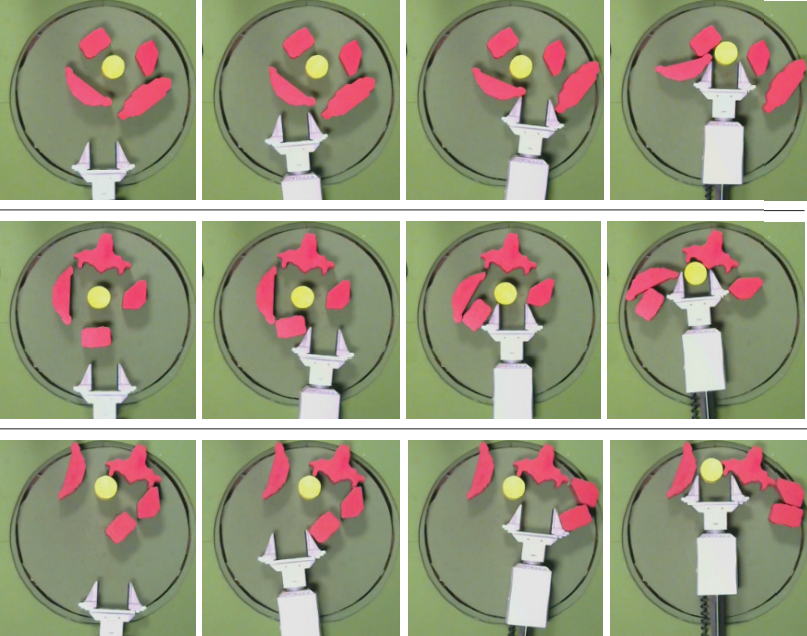
\includegraphics[width=0.5\textwidth]{f_figs/teaser.png}
\caption{
Three roll-outs on a Zymark 3-DOF Robot of a fully trained grasping in clutter policy (one per column, bottom to top) which was trained using a
hierarchy of three supervisors consisting of an analytical motion planning, crowd-sourcing and human expert. 
Red shapes indicate clutter objects and the robot is trained to reach the yellow circle. The trained manipulation policy is represented as a deep neural network that recieves as input an image of the scene and outputs a change in state position. The resulting policy learns to sweep away clutter objects and reach the goal object.  }
\vspace*{-20pt}
\label{fig:teaser}
\end{figure}

\section{Related Work}
Laskey et al. explored learning policies for the grasping in clutter problem based on image data, using a hierarchy of supervisors of different complexities to provide feedback to the robot ~\cite{hierarchical_supervisors}. The robot was trained using DAgger, an imitation learning method that iteratively rolls out a policy, incorporates feedback from the supervisors to expand the dataset, and retrains the policy ~\cite{ross2010reduction}. 

\section{Experiments} \label{sec:Exp}
\subsection{Robot System}
The robot, shown in Fig. 2, has a 3 dimensional
internal state of base rotation, arm extension and
gripper opening width. The state space of the environment is captured by an overhead Logitech C270 camera,
which is positioned to capture the workspace that contains
all cluttered objects, the goal object and the robot arm.
Examples of images from the camera can be seen in Fig.
1. The robot is commanded via position control with a PID
controller. The controls to the robot are
bounded changes in the internal state, which allows for us to
easily register control signals to the demonstrations provided
by supervisors as opposed to torque control. The control
signals for each degree of freedom are continuous values
with the following ranges: base rotation, $[-15^\circ
, 15^\circ]$, arm
extension $[-1, 1]$. The units are degrees for base rotation
and centimeters for arm extension. The precision of control
signal is 0.001 for each degree of freedom. 

\subsection{Expert Supervisor} 
As part of the problem formulation, we assume the existence of an expert supervisor, mapping the state space $X$ to the action space $U$, that performs the intended task well. An Expert Supervisor can utilize a variety of knowledge about the physical limitations of the robot and environment,
joint limits and experience in how certain objects might
behave under force ~\cite{ross2013learning}. Furthermore, the Expert Supervisor might
have an intuition for how training examples could lead to
better training of the robot.
The Expert Supervisor uses the interface shown in Fig. 3, to provide examples
to the robot.
\subsection{Neural Network Policy Architecture }
In Online LfD, a robot is trained by learning a policy, or function mapping state
space $X$ to control space $U$. To handle
the high dimensional image space of the problem, we are
interested in representing the robot’s policy as a deep neural
network. To facilitate training the neural network, we scaled the
controls between 1 and -1 for each dimension independently,
which is common for training ~\cite{tensorflow2015-whitepaper}. To be robust to lighting and
reduce the dimensionality of the problem, we applied a binary
mask to each channel of the 250x250 RGB images setting
values above 125 to one and 0 otherwise. The policy outputs
a 4 dimensional control signals, or delta state positions, for a
given input image or state. Our network architecture was designed as follows. First, to
work with image data we used a convolutional layer with 5
channels and 11x11 filters. Then we added a Rectified Linear
Unit (i.e. max(0, x)) or ReLu, to add a non-linearity between
layers. ReLus have been shown to allow for faster training
than other non-linear separators ~\cite{imagenet}. After the non-linearity
we added a fully connected layer, or a weight matrix with
an out dimension of 128. Then another ReLu followed by
a weight matrix that maps to the 4 dimensional output. We
place a final tanh function on the output, which enforces the
output is between −1 and 1.
We trained all networks on a dataset of 6K state/control pairs
from the MPIO Supervisor on a Nvidia Tesla K40 GPU,
which is able to train each network in an average of 10
minutes. All networks were trained using Stochastic Gradient
Descent with Momentum in TensorFlow ~\cite{tensorflow2015-whitepaper}. Momentum is
a method to control the magnitude of the gradient based on
how large previous gradients were. We used a gradient step
size,or learning rate of 0.01 and a momentum term of 0.9.

\subsection{Experimental Setup}
\begin{figure}[t]
\centering

\includegraphics[width=0.5\textwidth]{f_figs/robot.eps}

\caption{\footnotesize  Shown above is a Zymark robot. The robot consists of an 3DOF arm that lies in a planar workspace and the ability to rotate the turn table. The inscribed circle in the work space prevents the robot from learning the trivial policy of just pushing the objects off the table.}

\label{fig:robot}
\end{figure}

\begin{figure}[t]
\centering

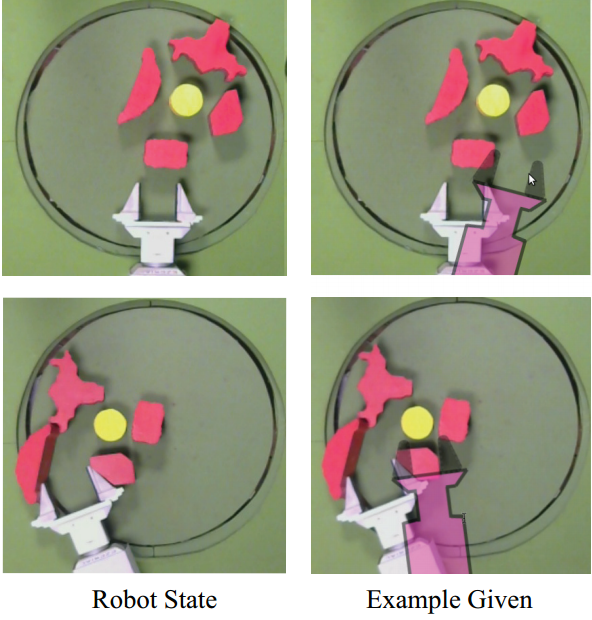
\includegraphics[width=0.5\textwidth]{f_figs/labeling_interface.png}

\caption{\footnotesize  The interface human supervisors see for providing feedback to the robot for the grasping in clutter task. The pink overlay indicates the desired 
control, which is a bounded change in internal state that the robot should apply.
Supervisors can then use their intuition for how objects respond to force
to provide examples of how the robot should behave. On the left side is
an example of a robot state and on the right side is an example a human
supervisor would provide via a computer mouse.}

\label{fig:labeling_interface}
\end{figure}

For the grasping in clutter task, we consider objects made
of Medium Density Fiberboard with an average 4” diameter
and 3” in height. The objects used to form clutter are red
extruded polygons while the goal object is a yellow cylinder.
The robot workspace, which is green, consists of a 30” disk
region which is surrounded by an elevated plate constraining
the objects to a ring and prohibiting them from leaving the
camera’s field of view.
To test the performance of each robot policy, we created
a test set composed of 20 different configurations each
containing objects that were not in the training set. The
training objects and test objects introduced during testing are
shown in Fig. 4. The test set configurations varied by placing
test objects from Fig. 4 with objects we trained on in similar
configurations. Examples of training and test configurations
are shown in Fig. 5. During training and testing, we manually
place the objects in configurations. However, a hardware
mechanism that moves the objects around, such as a predefined
sweeping motion from the robot arm, could be used
in future work. We measure success by whether the object
was in the gripper at the final timestep. We define reliability
or ρ as the percentage of successful configurations.
Per iteration of Hierarchical DAgger, we collect 20 trajectories
on different training configurations and then have a
supervisor provide 20 demonstrations. We do this to sample
a variety of configurations with the current policy before
updating the weights. Thus 100 robotic trials correspond to
5 iterations of DAgger.

\subsection{Image Filters}
In our experiments, we applied a variety of image filters to preprocess the images before training. The same filter was applied to the input to the neural net policy at runtime for experiments. \\
\textbf{Binary Mask (Original)}
The first filter was used for experiments in \textit{Hierarchical Supervisors}, and consisted of a binary mask applied to each channel of the 250x250 RGB images setting
values above 125 to one and 0 otherwise. \\
\\
\textbf{RGB}
The second approach used the raw RGB images directly. \\
\\
\textbf{Greyscale}
The third approach converted the raw RGB images to greyscale using OpenCV ~\cite{opencv}. 

\begin{figure}[t]
\centering

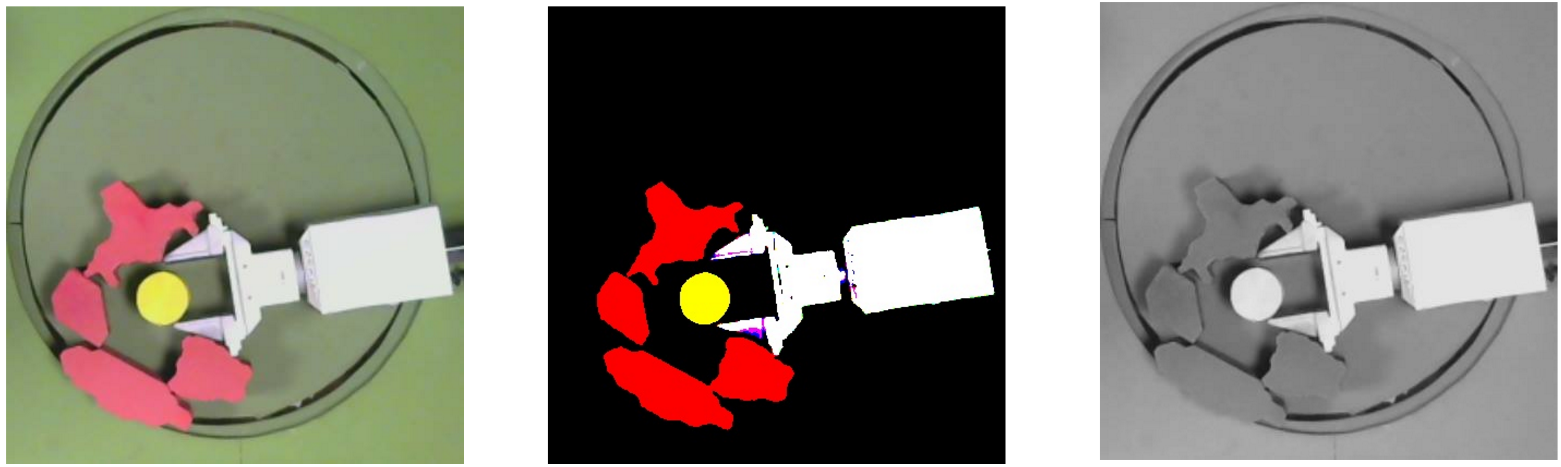
\includegraphics[width=0.5\textwidth]{f_figs/image_filters.png}

\caption{\footnotesize Visualization of the application of different image filters to a target image. From left to right, the filters are: binary mask, RGB, greyscale.}

\label{fig:image_filters}
\end{figure}

\subsection{Net Architectures}
We experimented with three different neural network architectures.  We trained each of these nets with DAgger, using 100 rollouts labeled by an expert human supervisor. \\
\\
\textbf{Fully Connected}
The first architecture was used for experiments in \textit{Hierarchical Supervisors}, and consisted of a convolutional layer with 5 channels and 11x11 filters.  This was followed by a Rectified Linear Unit, or ReLu, for non-linearity.  Next, was a fully connected layer with an out dimension of 128, followed by another ReLu and a weight matrix.  The final part is a tanh for the output. \\
\\
\textbf{Max Pooling}
The second architecture we used was a variation on the first architecture, with the addition of a max pooling layer of kernel size 4 after the first convolutional layer. \\
\\
\textbf{Convolutional Layer}
The third architecture was also a variation on the first architecture, with the addition of an identical convolutional layer after the first convolutional layer.

\subsection{Metrics}
We evaluate the performance of a policy rollout on its final state.
We quantify our results using the L2 distance between the gripper and golden circle, as well as a binary measurement of successful grasp. To automatically locate the target object and the gripper in the image, we used template matching, implemented in OpenCV, which uses a cross-correlation filter and a set of target object and gripper object image files.  

\subsection{Results}
After training on the initial data, we evaluated our policy on similar grasping problems. We train on a smaller dataset than in the hierarchical supervisors paper;  we achieve lower absolute rewards, but experimentally demonstrate significant differences between the rewards of the different setups. 

From these results, we find that applying the binary mask filter results in the best relative performance. RGB and greyscale filters return similar performance.
The fully connected layer used in the paper returns similar performance to that of the max pooling layer using both metrics of performance. Adding another convolutional layer greatly degrades performance.

\begin{figure}[t]
\centering

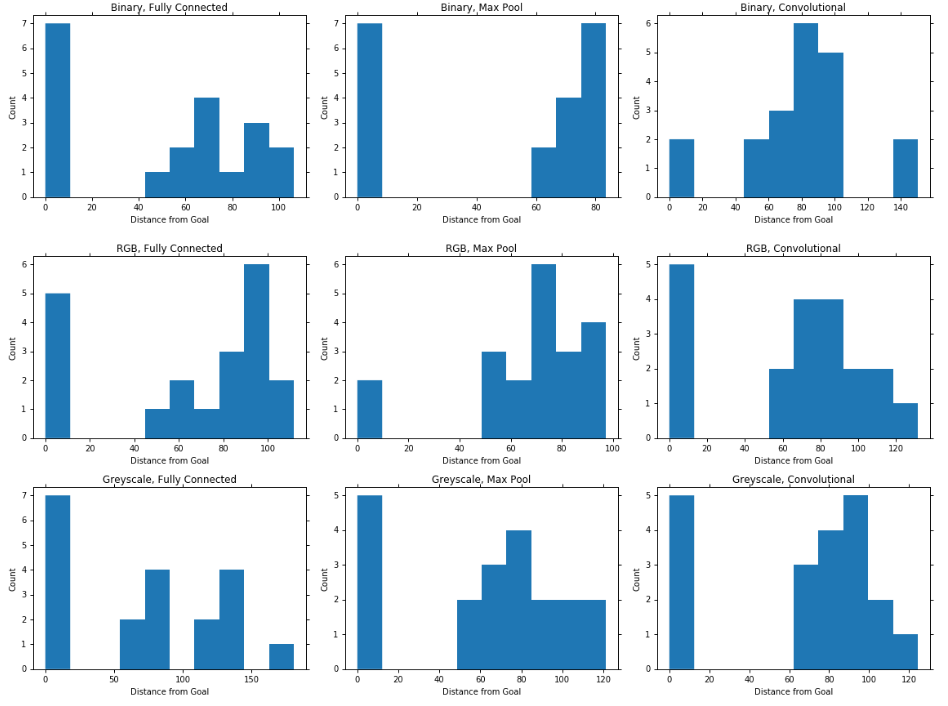
\includegraphics[width=0.5\textwidth]{f_figs/results_histograms.png}

\caption{\footnotesize Histograms of final distances between the gripper and target object in 20 trials for each possible net and filter combination.}

\label{fig:results_histograms}
\end{figure}

\begin{figure}[t]
\centering

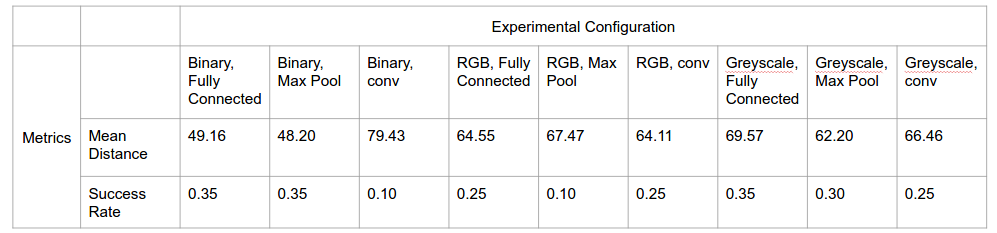
\includegraphics[width=0.5\textwidth]{f_figs/results_tables.png}

\caption{\footnotesize Table of success rates for grasping the target object in 20 trials for each possible net and filter combination.}

\label{fig:results_tables}
\end{figure}

\section{Discussions and Future Work}
Future possible experiments include usage of alternative supervisors to provide feedback to the robot during training, such as reinforcement learning methods. In particular, policy gradient methods provide a possible way to perform training tasks without continuous human feedback. Another possibility is exploring different net architectures, such as spatial softmax layers or recurrent neural networks.

\section{Acknowledgments} 
We thank Michael Laskey and Ken Goldberg for guidance and contributing software and equipment for this project. 
  
\bibliographystyle{IEEEtranS}
\bibliography{references}



\end{document}